\subsection{Flip-Flop T}

O flip-flop T (\textit{Toggle}) é um elemento elemento de memória specializado na alternância de estado. Ele é amplamente utilizado na construção de contadores e divisores de frequência.

Entrada:
\begin{itemize}
    \item $T$ : Toggle
\end{itemize}

\begin{center}
\begin{tabular}{c | c}
T & $Q_{t+1}$ \\
\hline
0 & $Q_t$ \\
1 & $\overline{Q_t}$
\end{tabular}
\end{center}

Ou seja, quando $T = 1$, o estado é invertido a cada borda ativa do clock. Quando $T = 0$, o estado é mantido.

Esse comportamento pode ser expresso de forma compacta como:

\[
Q_{t+1} = T \oplus Q_t
\]

Uma forma comum de implementação do flip-flop T é a partir de um flip-flop JK, conectando-se as entradas $J$ e $K$ ao sinal $T$:

\[
J = K = T
\]

\begin{figure}[H]
    \centering
    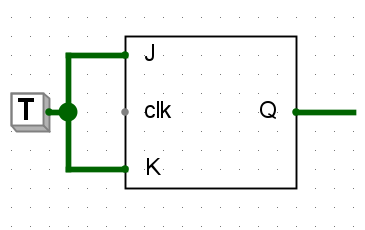
\includegraphics[width=0.5\linewidth]{images/T-FF-circuit.png}
    \caption{Implementação do Flip Flop tipo T a partir do Flip Flop JK}
    \label{fig:T-FF-circuit}
\end{figure}

Nesse arranjo, quando $T = 1$, o circuito entra no modo de alternância, enquanto $T = 0$ preserva o estado atual.

Uma aplicação fundamental do flip-flop T é como divisor de frequência. Quando $T = 1$ constantemente, o sinal de saída $Q$ alterna a cada ciclo de clock, resultando em uma frequência de saída igual à metade da frequência de entrada:

\begin{figure}[H]
    \centering
    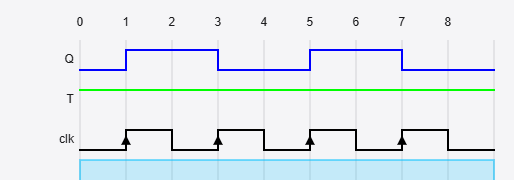
\includegraphics[width=0.8\linewidth]{images/T-FF-freq-half.png}
    \caption{Diagrama Temporal de Q por clock com $T=1$}
    \label{fig:T-FF-freq-half}
\end{figure}

\[
f_{out} = \frac{f_{clk}}{2}
\]

Além disso, esse comportamento permite a construção de contadores binários, que serão abordados na sessão \textbf{4.5}.

\begin{figure}[H]
    \centering
    \includegraphics[width=0.5\linewidth]{images/T-FF-redstone.png}
    \caption{Implementação do Flip Flop tipo T a partir do Flip Flop JK, em redstone.}
    \label{fig:T-FF-redstone}
\end{figure}